%
% This document contains the chapter about S-parameters.
%
% Copyright (C) 2003, 2004 Stefan Jahn <stefan@lkcc.org>
% Copyright (C) 2004 Michael Margraf <Michael.Margraf@alumni.TU-Berlin.DE>
%
% Permission is granted to copy, distribute and/or modify this document
% under the terms of the GNU Free Documentation License, Version 1.1
% or any later version published by the Free Software Foundation.
%

\chapter{Scattering parameters}
%\addcontentsline{toc}{chapter}{Scattering parameters}

\section{Introduction and definition}
%\addcontentsline{toc}{section}{Introduction and definition}

Voltage and current are hard to measure at high frequencies.  Short
and open circuits (used by definitions of most n-port parameters) are
hard to realize at high frequencies.  Therefore, microwave engineers
work with so-called scattering parameters (S parameters), that uses
waves and matched terminations (normally $50 \Omega$).  This procedure
also minimizes reflection problems.

\addvspace{12pt}

A (normalized) wave is defined as ingoing wave $\underline{a}$ or
outgoing wave $\underline{b}$:

\begin{equation}
\underline{a} = \frac{u+Z_0\cdot i}{\sqrt{\text{Re}(Z_0)}} \qquad
\underline{b} = \frac{u-Z_0^*\cdot i}{\sqrt{\text{Re}(Z_0)}}
\label{equ:waves}
\end{equation}
where $u$ is (effective) voltage, $i$ (effective) current and $Z_0$ reference
impedance. The waves are related to power in the following way.
\begin{equation}
P = \left( |\underline{a}|^2 - |\underline{b}|^2 \right)
\end{equation}
Sometimes waves are defined with peak voltages and peak currents.
The only difference that appears then is the relation to power:
\begin{equation}
P = \frac{1}{2}\cdot \left( |\underline{a}|^2 - |\underline{b}|^2 \right)
\end{equation}
Now, characterizing an n-port is straight-forward:
\begin{equation}
\begin{pmatrix}
\underline{b}_1\\
\vdots\\
\underline{b}_n\\
\end{pmatrix}
=
\begin{pmatrix}
\underline{S}_{11} & \ldots & \underline{S}_{1n}\\
\vdots & \ddots & \vdots\\
\underline{S}_{n1} & \ldots & \underline{S}_{nn}\\
\end{pmatrix}
\cdot
\begin{pmatrix}
\underline{a}_1\\
\vdots\\
\underline{a}_n\\
\end{pmatrix}
\end{equation}


\section{Computing with S-parameters}
%\addcontentsline{toc}{section}{Computing with S-parameters}

\subsection{Recalculating $\mathbf{50\ohm}$-S-parameters for arbitrary port impedances}
%\addcontentsline{toc}{subsection}{Recalculating $50\ohm$-S-parameters for arbitrary port impedances}

During S-parameter usage it sometimes appears to have not all components
in a circuit normalized to the same impedance. But calculations can only
be performed with all ports being normalized to the same impedance. In
the field of high
frequency techniques this is usually $50\ohm$.  In order to transform
to different port impedances, the following computation must be applied
to the resulting S-parameter matrix.

\begin{equation}
\left[\underline{N'}\right] =
\left(\left[\underline{S}\right] - \left[\underline{R}\right]\right) \cdot
\left(\left[\underline{E}\right] - \left[\underline{R}\right] \cdot \left[\underline{S}\right]\right)^{-1}
\end{equation}

\begin{equation}
\underline{N}_{nm} = \underline{N'}_{nm}\cdot \sqrt{\dfrac{Z_m}{Z_n}\cdot
\dfrac{Z_{n,before}}{Z_{m,before}}}\cdot
\dfrac{Z_n + Z_{n,before}}{Z_m + Z_{m,before}}
\end{equation}

With

\addvspace{12pt}

\begin{tabular}{rll}
$Z_{n}$ & = & norm impedance after the normalizing process\\& &\\
$Z_{n,before}$ & = & norm impedance before the normalizing process\\& &\\
$\left[\underline{E}\right]$ & = &
$\begin{pmatrix}
1 & 0 & \ldots & 0\\
0 & 1 & \ldots & 0\\
\vdots & \vdots & \ddots & \vdots\\
0 & 0 & \ldots & 1\\
\end{pmatrix}$
identity matrix\\& &\\
$\left[\underline{S}\right]$ & = & original $50\ohm$-S-parameter matrix\\& &\\
$\left[\underline{N}\right]$ & = & recalculated scattering matrix\\& &\\
$\left[\underline{R}\right]$ & = &
$\begin{pmatrix}
\underline{r}(Z_{1}) & 0 & \ldots & 0\\
0 & \underline{r}(Z_{2}) & \ldots & 0\\
\vdots & \vdots & \ddots & \vdots\\
0 & 0 & \ldots & \underline{r}(Z_{n})\\
\end{pmatrix}$
reflection coefficient matrix\\& &\\
$\underline{r}(Z_{n})$ & = &
$\dfrac{Z_{n} - Z_{n,before}}{Z_{n} + Z_{n,before}}$
reflection coefficient of impedance at port n\\& &\\
\end{tabular}

And furthermore

\addvspace{12pt}

\begin{tabular}{rll}
$\left[\underline{X}\right]^{-1}$ & = & 
inverted matrix of $\left[\underline{X}\right]$\\& &\\
$\underline{X}_{nm}$ & = & 
element of matrix $\left[\underline{X}\right]$ at row n and column m\\& &\\
\end{tabular}

\subsection{S-parameters in CAE programs}
%\addcontentsline{toc}{subsection}{S-parameters in CAE programs}
\label{sec:SparameterCAE}

The most common task of a simulation program is to compute the S
parameters of an arbitrary network that consists of many elementary
components connected to each other.  To perform this, one can build a
large matrix containing the S parameters of all components and then
use matrix operations to solve it.  However this method needs heavy
algorithms.  A more elegant possibility was published in
\cite{Compton}. Each step computes only one connection and so unites
two connected components to a single S parameter block.  This
procedure has to be done with every connection until there is only one
block left whose S parameters therefore are the simulation result.

\addvspace{12pt}

Connecting port $k$ of circuit $(\underline{S})$ with port $l$ of
circuit $(\underline{T})$, the new S-parameters are
\begin{equation}
\underline{S}'_{ij} = \underline{S}_{ij} +
      \frac{\underline{S}_{kj}\cdot \underline{T}_{ll}\cdot \underline{S}_{ik}}
           {1-\underline{S}_{kk}\cdot \underline{T}_{ll}}
\label{eq:connectSij}
\end{equation}
with $i$ and $j$ both being ports of $(\underline{S})$.  Furthermore, it is
\begin{equation}
\underline{S}'_{mj} =
      \frac{\underline{S}_{kj}\cdot \underline{T}_{ml}}
           {1-\underline{S}_{kk}\cdot \underline{T}_{ll}}
\label{eq:connectSmj}
\end{equation}
with $m$ being a port of the circuit $(\underline{T})$.  If two ports
of the same circuit $(\underline{S})$ are connected, the new
S-parameters are
\begin{equation}
\underline{S}'_{ij} = \underline{S}_{ij} +
      \frac{ \underline{S}_{kj}\cdot \underline{S}_{il}\cdot (1-\underline{S}_{lk})
           + \underline{S}_{lj}\cdot \underline{S}_{ik}\cdot (1-\underline{S}_{kl})
           + \underline{S}_{kj}\cdot \underline{S}_{ll}\cdot \underline{S}_{ik}
           + \underline{S}_{lj}\cdot \underline{S}_{kk}\cdot \underline{S}_{il}}
           {(1-\underline{S}_{kl})\cdot (1-\underline{S}_{lk}) - \underline{S}_{kk}\cdot \underline{S}_{ll}}.
\label{eq:iconnectSij}
\end{equation}

The formulas \eqref{eq:connectSij}, \eqref{eq:connectSmj} and
\eqref{eq:iconnectSij} are obtained using the ``nontouching-loop''
rule being an analytical method for solving a flow graph.  A few basic
definitions have to be understood.

\addvspace{12pt}

A ``path'' is a series of branches into the same direction with no
node touched more than once.  A paths value is the product of the
coefficients of the branches.  A ``loop'' is formed when a path starts
and finishes at the same node.  A ``first-order'' loop is a path
coming to closure with no node passed more than once.  Its value is
the product of the values of all branches encountered on the route.  A
``second-order'' loop consists of two first-order loops not touching
each other at any node.  Its value is calculated as the product of the
values of the two first-order loops.  Third- and higher-order loops
are three or more first-order loops not touching each other at any
node.

\addvspace{12pt}

The nontouching-loop rule can be applied to solve any flow graph.  In
the following equation in symbolic form $T$ represents the ratio of
the dependent variable in question and the independent variable.

\begin{equation}
T = \dfrac{
\begin{array}{r}
P_{1}\cdot\left(1 - \Sigma L_{1}^{(1)} + \Sigma L_{2}^{(1)} - \Sigma L_{3}^{(1)} + \ldots\right) +
P_{2}\cdot\left(1 - \Sigma L_{1}^{(2)} + \Sigma L_{2}^{(2)} - \Sigma L_{3}^{(2)} + \ldots\right)\\
+ P_{3}\cdot\left(1 - \Sigma L_{1}^{(3)} + \Sigma L_{2}^{(3)} - \Sigma L_{3}^{(3)} + \ldots\right) +
P_{4}\cdot\left(1 - \ldots\right) + \ldots
\end{array}
}{1 - \Sigma L_{1} + \Sigma L_{2} - \Sigma L_{3} + \ldots}
\label{eq:ntrule}
\end{equation}

In eq. \eqref{eq:ntrule} $\Sigma L_{1}$ stands for the sum of all
first-order loops, $\Sigma L_{2}$ is the sum of all second-order
loops, and so on.  $P_{1}$, $P_{2}$, $P_{3}$ etc., stand for the
values of all paths that can be found from the independent variable to
the dependent variable.  $\Sigma L_{1}^{(1)}$ denotes the sum of those
first-order loops which do not touch (hence the name) the path of
$P_{1}$ at any node, $\Sigma L_{2}^{(1)}$ denotes then the sum of
those second-order loops which do not touch the path $P_{1}$ at any
point, $\Sigma L_{1}^{(2)}$ consequently denotes the sum of those
first-order loops which do not touch the path of $P_{2}$ at any point.
Each path is multiplied by the factor in parentheses which involves
all the loops of all orders that the path does not touch.

\addvspace{12pt}

When connecting two different networks the signal flow graph in
fig. \ref{fig:sconnectgraph} is used to compute the new S-parameters.
With equally reference impedances on port $k$ and port $l$ the
relations $\underline{a}_{k} = \underline{b}_{l}$ and
$\underline{a}_{l} = \underline{b}_{k}$ are satisfied.

\begin{figure}[ht]
\begin{center}
\includegraphics[width=0.8\linewidth]{sconnectgraph}
\end{center}
\caption{signal flow graph of a joint between ports $k$ and $l$ on different networks}
\label{fig:sconnectgraph}
\end{figure}
\FloatBarrier

There is only one first-order loop (see fig. \ref{fig:sconnectloop})
within this signal flow graph.  This loops value yields to
\begin{equation}
L_{11} = \underline{S}_{kk}\cdot \underline{T}_{ll}
\end{equation}

\begin{figure}[ht]
\begin{center}
\includegraphics[height=3.1cm]{sconnectloop}
\end{center}
\caption{loops in the signal flow graph when connecting ports $k$ and $l$ on different networks}
\label{fig:sconnectloop}
\end{figure}
\FloatBarrier

The paths that can be found from the independent variable
$\underline{a}_{j}$ to the dependent variable $\underline{b}_{i}$ (as
depicted in fig. \ref{fig:sconnectpath}) can be written as
\begin{align}
P_{1} &= \underline{S}_{kj}\cdot \underline{T}_{ll} \cdot \underline{S}_{ik}\\
P_{2} &= \underline{S}_{ij}
\end{align}

\begin{figure}[ht]
\begin{center}
\includegraphics[height=3.1cm]{sconnectpath}
\end{center}
\caption{paths in the signal flow graph when connecting ports $k$ and $l$ on different networks}
\label{fig:sconnectpath}
\end{figure}
\FloatBarrier

Applying the nontouching-loop rule, i.e. eq. \eqref{eq:ntrule}, gives
the new S-parameter $\underline{S}'_{ij}$
\begin{equation}
\begin{split}
\underline{S}'_{ij} = \dfrac{\underline{b}_{i}}{\underline{a}_{j}} &= \dfrac{P_{1}\cdot\left(1 - L_{11}\right) + P_{2}\cdot 1}{1 - L_{11}}\\
&= \dfrac{\underline{S}_{ij}\cdot\left(1 - \underline{S}_{kk}\cdot \underline{T}_{ll}\right) + \underline{S}_{kj}\cdot \underline{T}_{ll}\cdot \underline{S}_{ik}}{1 - \underline{S}_{kk}\cdot \underline{T}_{ll}}
= \underline{S}_{ij} + \dfrac{\underline{S}_{kj}\cdot \underline{T}_{ll}\cdot \underline{S}_{ik}}{1 - \underline{S}_{kk}\cdot \underline{T}_{ll}}
\end{split}
\end{equation}

The only path that can be found from the independent variable
$\underline{a}_{j}$ to the dependent variable $\underline{b}_{m}$ (as
depicted in fig. \ref{fig:sconnectpath}) can be written as
\begin{equation}
P_{1} = \underline{S}_{kj}\cdot \underline{T}_{ml}
\end{equation}

Thus the new S-parameter $\underline{S}'_{mj}$ yields to
\begin{equation}
\underline{S}'_{mj} = \dfrac{\underline{b}_{m}}{\underline{a}_{j}}
= \dfrac{P_{1}\cdot 1}{1 - L_{11}}
= \dfrac{\underline{S}_{kj}\cdot \underline{T}_{ml}}{1 - \underline{S}_{kk}\cdot \underline{T}_{ll}}
\end{equation}

When connecting the same network the signal flow graph in
fig. \ref{fig:siconnectgraph} is used to compute the new S-parameters.
With equally reference impedances on port $k$ and port $l$ the
relations $\underline{a}_{k} = \underline{b}_{l}$ and
$\underline{a}_{l} = \underline{b}_{k}$ are satisfied.

\begin{figure}[ht]
\begin{center}
\includegraphics[width=0.55\linewidth]{siconnectgraph}
\end{center}
\caption{signal flow graph of a joint between ports $k$ and $l$ on the same network}
\label{fig:siconnectgraph}
\end{figure}
\FloatBarrier

There are three first-order loops and a second-order loop (see
fig. \ref{fig:siconnectloop}) within this signal flow graph.  These
loops' values yield to
\begin{align}
L_{11} &= \underline{S}_{kk}\cdot \underline{S}_{ll}\\
L_{12} &= \underline{S}_{kl}\\
L_{13} &= \underline{S}_{lk}\\
L_{21} &= L_{12}\cdot L_{13} = \underline{S}_{kl}\cdot \underline{S}_{lk}
\end{align}

\begin{figure}[ht]
\begin{center}
\includegraphics[height=3.7cm]{siconnectloop}
\end{center}
\caption{loops in the signal flow graph when connecting ports $k$ and $l$ on the same network}
\label{fig:siconnectloop}
\end{figure}
\FloatBarrier

There are five different paths that can be found from the independent
variable $\underline{a}_{j}$ to the dependent variable
$\underline{b}_{i}$ (as depicted in fig. \ref{fig:siconnectpath})
which can be written as
\begin{align}
P_{1} &= \underline{S}_{kj}\cdot \underline{S}_{ll}\cdot \underline{S}_{ik}\\
P_{2} &= \underline{S}_{kj}\cdot \underline{S}_{il}\\
P_{3} &= \underline{S}_{lj}\cdot \underline{S}_{ik}\\
P_{4} &= \underline{S}_{ij}\\
P_{5} &= \underline{S}_{lj}\cdot \underline{S}_{kk}\cdot \underline{S}_{il}
\end{align}

\begin{figure}[ht]
\begin{center}
\includegraphics[height=7.4cm]{siconnectpath}
\end{center}
\caption{paths in the signal flow graph when connecting ports $k$ and $l$ on the same network}
\label{fig:siconnectpath}
\end{figure}
\FloatBarrier

Thus the new S-parameter $\underline{S}'_{ij}$ yields to
\begin{equation}
\begin{split}
\underline{S}'_{ij}
&= \dfrac{P_{1} + P_{2}\cdot\left(1 - L_{13}\right) + P_{3}\cdot\left(1 - L_{12}\right) + P_{4}\cdot\left(1 - \left(L_{11} + L_{12} + L_{13}\right) + L_{21}\right) + P_{5}}{1 - \left(L_{11} + L_{12} + L_{13}\right) + L_{21}}\\
&= P_{4} + \dfrac{P_{1} + P_{2}\cdot\left(1 - L_{13}\right) + P_{3}\cdot\left(1 - L_{12}\right) + P_{5}}{1 - \left(L_{11} + L_{12} + L_{13}\right) + L_{21}}\\
&= \underline{S}_{ij} + \dfrac{\underline{S}_{kj}\cdot \underline{S}_{ll}\cdot \underline{S}_{ik} + \underline{S}_{kj}\cdot \underline{S}_{il} \cdot\left(1 - \underline{S}_{lk}\right) + \underline{S}_{lj}\cdot \underline{S}_{ik}\cdot\left(1 - \underline{S}_{kl}\right) + \underline{S}_{lj}\cdot \underline{S}_{kk}\cdot \underline{S}_{il}}{1 - \left(\underline{S}_{kk}\cdot \underline{S}_{ll} + \underline{S}_{kl} + \underline{S}_{lk}\right) + \underline{S}_{kl}\cdot \underline{S}_{lk}}\\
&= \underline{S}_{ij} + \dfrac{\underline{S}_{kj}\cdot \underline{S}_{ll}\cdot \underline{S}_{ik} + \underline{S}_{kj}\cdot \underline{S}_{il} \cdot\left(1 - \underline{S}_{lk}\right) + \underline{S}_{lj}\cdot \underline{S}_{ik}\cdot\left(1 - \underline{S}_{kl}\right) + \underline{S}_{lj}\cdot \underline{S}_{kk}\cdot \underline{S}_{il}}{\left(1 - \underline{S}_{kl}\right)\cdot \left(1 - \underline{S}_{lk}\right) - \underline{S}_{kk}\cdot \underline{S}_{ll}}
\end{split}
\end{equation}

This short introduction to signal flow graphs and their solution using
the nontouching-loop rule verifies the initial formulas used to
compute the new S-parameters for the reduced subnetworks.

\addvspace{12pt}

If more than two ports are connected at a node, one have to insert a
tee.  Its S-parameters write as follows.
\begin{equation}
\begin{pmatrix}
\underline{S}
\end{pmatrix}
= \dfrac{1}{3}\cdot
\begin{pmatrix}
-1 &  2 &  2\\
 2 & -1 &  2\\
 2 &  2 & -1\\
\end{pmatrix}
\end{equation}


\subsection{Differential S-parameter ports}
%\addcontentsline{toc}{subsection}{Differential S-parameter ports}
\label{sec:diffSParam}

The implemented algorithm for the S-parameter analysis calculates
S-parameters in terms of the ground node.  In order to allow
differential S-parameters as well it is necessary to insert an ideal
impedance transformer with a turns ratio of 1:1 between the
differential port and the device under test.

\begin{figure}[ht]
\begin{center}
\includegraphics[width=12cm]{differential}
\end{center}
\caption{transformation of differential port into single ended port}
\label{fig:differential}
\end{figure}
\FloatBarrier

The S-parameter matrix of the inserted ideal transformer being a three
port device can be written as follows.

\begin{equation}
\begin{pmatrix}
\underline{S}
\end{pmatrix}
= \dfrac{1}{3}\cdot
\begin{pmatrix}
1 & 2 & -2\\
2 & 1 & 2\\
-2 & 2 & 1\\
\end{pmatrix}
\end{equation}

This transformation can be applied to each S-parameter port in a
circuit regardless whether it is actually differential or not.

\addvspace{12pt}

It is also possible to do the impedance transformation within this step
(for S-parameter ports with impedances different than $50\ohm$). This can
be done by using a transformer with an impedance ration of

\begin{equation}
r=T^2=\frac{50\ohm}{Z}
\end{equation}

With $Z$ being the S-parameter port impedance. The S-parameter matrix of
the inserted ideal transformer now writes as follows.

\begin{equation}
\begin{pmatrix}
\underline{S}
\end{pmatrix}
= \dfrac{1}{2\cdot Z_0+Z}\cdot
\begin{pmatrix}
2\cdot Z_0-Z              & 2\cdot\sqrt{Z_0\cdot Z}  & -2\cdot\sqrt{Z_0\cdot Z}\\
2\cdot\sqrt{Z_0\cdot Z}   & Z                        & 2\cdot Z_0\\
-2\cdot\sqrt{Z_0\cdot Z}  & 2\cdot Z_0               & Z\\
\end{pmatrix}
\end{equation}

With $Z$ being the new S-parameter port impedance and $Z_0$ being $50\ohm$.

\section{Matrix conversions}
%\addcontentsline{toc}{section}{Matrix conversions}
\label{sec:SparameterConversion}

When dealing with S-parameter analyses it may be necessary or
convenient to convert the resulting scattering parameter matrix into
other matrix representations used in microwave engineering.

\subsection{S-Parameter to impedance matrix}
%\addcontentsline{toc}{subsection}{S-Parameter to impedance matrix}

Converting a scattering parameter matrix to an impedance matrix is
done by the following formula.

\begin{equation}
\left[
\underline{Z}
\right]
=
\left[
\underline{G}_{ref}
\right]^{-1}
\cdot
\left(
\left[\underline{E}\right] - \left[\underline{S}\right]
\right)^{-1}
\cdot
\left(
\left[\underline{S}\right] \cdot \left[\underline{Z}_{ref}\right] + \left[\underline{Z}_{ref}\right]^{*}
\right)
\cdot
\left[\underline{G}_{ref}\right]
\end{equation}

With

\addvspace{12pt}

\begin{tabular}{rll}
$\left[\underline{E}\right]$ & = &
$\begin{bmatrix}
1 & 0 & \ldots & 0\\
0 & 1 & \ldots & 0\\
\vdots & \vdots & \ddots & \vdots\\
0 & 0 & \ldots & 1\\
\end{bmatrix}$
identity matrix\\& &\\
$\left[\underline{S}\right]$ & = & original S-parameter matrix\\& &\\
$\left[\underline{Z}\right]$ & = & resulting impedance matrix\\& &\\
$\left[\underline{Z}_{ref}\right]$ & = &
$\left[\underline{E}\right] \cdot Z_{0}$\\& &\\
$\left[\underline{G}_{ref}\right]$ & = &
$\left[\underline{E}\right] \cdot 
\dfrac{1}{2\cdot \sqrt{\left| \text{Re}\left(Z_{0}\right)\right|}}$\\& &\\
$Z_{0}$ & = & reference impedance (by default $50\ohm$)\\& &\\
\end{tabular}

And furthermore

\addvspace{12pt}

\begin{tabular}{rll}
$\left[\underline{X}\right]^{-1}$ & = & 
inverted matrix of $\left[\underline{X}\right]$\\& &\\
$\left[\underline{X}\right]^{*}$ & = & 
complex conjugated matrix of $\left[\underline{X}\right]$\\& &\\
\end{tabular}

\subsection{S-Parameter to admittance matrix}
%\addcontentsline{toc}{subsection}{S-Parameter to admittance matrix}

Converting a scattering parameter matrix to an admittance matrix can
be achieved by computing the following formula.

\begin{equation}
\left[
\underline{Y}
\right]
=
\left[
\underline{G}_{ref}
\right]^{-1}
\cdot
\left(
\left[\underline{S}\right] \cdot \left[\underline{Z}_{ref}\right] + \left[\underline{Z}_{ref}\right]^{*}
\right)^{-1}
\cdot
\left(
\left[\underline{E}\right] - \left[\underline{S}\right]
\right)
\cdot
\left[\underline{G}_{ref}\right]
\end{equation}

With

\addvspace{12pt}

\begin{tabular}{rll}
$\left[\underline{E}\right]$ & = &
$\begin{bmatrix}
1 & 0 & \ldots & 0\\
0 & 1 & \ldots & 0\\
\vdots & \vdots & \ddots & \vdots\\
0 & 0 & \ldots & 1\\
\end{bmatrix}$
identity matrix\\& &\\
$\left[\underline{S}\right]$ & = & original S-parameter matrix\\& &\\
$\left[\underline{Y}\right]$ & = & resulting admittance matrix\\& &\\
$\left[\underline{Z}_{ref}\right]$ & = &
$\left[\underline{E}\right] \cdot Z_{0}$\\& &\\
$\left[\underline{G}_{ref}\right]$ & = &
$\left[\underline{E}\right] \cdot 
\dfrac{1}{2\cdot \sqrt{\left| \text{Re}\left(Z_{0}\right)\right|}}$\\& &\\
$Z_{0}$ & = & reference impedance (by default $50\ohm$)\\& &\\
\end{tabular}

And furthermore

\addvspace{12pt}

\begin{tabular}{rll}
$\left[\underline{X}\right]^{-1}$ & = & 
inverted matrix of $\left[\underline{X}\right]$\\& &\\
$\left[\underline{X}\right]^{*}$ & = & 
complex conjugated matrix of $\left[\underline{X}\right]$\\& &\\
\end{tabular}

\subsection{Impedance matrix to scattering parameter matrix}
%\addcontentsline{toc}{subsection}{Impedance matrix to scattering parameter matrix}

Converting an impedance matrix to a scattering parameter matrix is
done by the following formula.

\begin{equation}
\left[
\underline{S}
\right]
=
\left[
\underline{G}_{ref}
\right]
\cdot
\left(
\left[\underline{Z}\right] - \left[\underline{Z}_{ref}\right]^{*}
\right)
\cdot
\left(
\left[\underline{Z}\right] + \left[\underline{Z}_{ref}\right]
\right)^{-1}
\cdot
\left[\underline{G}_{ref}\right]^{-1}
\end{equation}

With

\addvspace{12pt}

\begin{tabular}{rll}
$\left[\underline{E}\right]$ & = &
$\begin{bmatrix}
1 & 0 & \ldots & 0\\
0 & 1 & \ldots & 0\\
\vdots & \vdots & \ddots & \vdots\\
0 & 0 & \ldots & 1\\
\end{bmatrix}$
identity matrix\\& &\\
$\left[\underline{S}\right]$ & = & resulting S-parameter matrix\\& &\\
$\left[\underline{Z}\right]$ & = & original impedance matrix\\& &\\
$\left[\underline{Z}_{ref}\right]$ & = &
$\left[\underline{E}\right] \cdot Z_{0}$\\& &\\
$\left[\underline{G}_{ref}\right]$ & = &
$\left[\underline{E}\right] \cdot 
\dfrac{1}{2\cdot \sqrt{\left| \text{Re}\left(Z_{0}\right)\right|}}$\\& &\\
$Z_{0}$ & = & reference impedance (by default $50\ohm$)\\& &\\
\end{tabular}

And furthermore

\addvspace{12pt}

\begin{tabular}{rll}
$\left[\underline{X}\right]^{-1}$ & = &
inverted matrix of $\left[\underline{X}\right]$\\& &\\
$\left[\underline{X}\right]^{*}$ & = & 
complex conjugated matrix of $\left[\underline{X}\right]$\\& &\\
\end{tabular}

\subsection{Admittance matrix to scattering parameter matrix}
%\addcontentsline{toc}{subsection}{Admittance matrix to scattering parameter matrix}

Converting an admittance matrix to a scattering parameter matrix is
done by the following formula.

\begin{equation}
\left[
\underline{S}
\right]
=
\left[
\underline{G}_{ref}
\right]
\cdot
\left(
\left[\underline{E}\right] - \left[\underline{Z}_{ref}\right]^{*} \cdot \left[\underline{Y}\right]
\right)
\cdot
\left(
\left[\underline{E}\right] + \left[\underline{Z}_{ref}\right] \cdot \left[\underline{Y}\right]
\right)^{-1}
\cdot
\left[\underline{G}_{ref}\right]^{-1}
\end{equation}

With

\addvspace{12pt}

\begin{tabular}{rll}
$\left[\underline{E}\right]$ & = &
$\begin{bmatrix}
1 & 0 & \ldots & 0\\
0 & 1 & \ldots & 0\\
\vdots & \vdots & \ddots & \vdots\\
0 & 0 & \ldots & 1\\
\end{bmatrix}$
identity matrix\\& &\\
$\left[\underline{S}\right]$ & = & resulting S-parameter matrix\\& &\\
$\left[\underline{Y}\right]$ & = & original admittance matrix\\& &\\
$\left[\underline{Z}_{ref}\right]$ & = &
$\left[\underline{E}\right] \cdot Z_{0}$\\& &\\
$\left[\underline{G}_{ref}\right]$ & = &
$\left[\underline{E}\right] \cdot 
\dfrac{1}{2\cdot \sqrt{\left| \text{Re}\left(Z_{0}\right)\right|}}$\\& &\\
$Z_{0}$ & = & reference impedance (by default $50\ohm$)\\& &\\
\end{tabular}

And furthermore

\addvspace{12pt}

\begin{tabular}{rll}
$\left[\underline{X}\right]^{-1}$ & = & 
inverted matrix of $\left[\underline{X}\right]$\\& &\\
$\left[\underline{X}\right]^{*}$ & = & 
complex conjugated matrix of $\left[\underline{X}\right]$\\& &\\
\end{tabular}

\subsection{Impedance matrix to admittance matrix}
%\addcontentsline{toc}{subsection}{Impedance matrix to admittance matrix}

Converting an impedance matrix to an admittance matrix is done by the
following formula.

\begin{equation}
\left[
\underline{Y}
\right]
=
\left[
\underline{Z}
\right]^{-1}
\end{equation}

With

\addvspace{12pt}

\begin{tabular}{rll}
$\left[\underline{Y}\right]$ & = & resulting admittance matrix\\& &\\
$\left[\underline{Z}\right]$ & = & original impedance matrix\\& &\\
\end{tabular}

And furthermore

\addvspace{12pt}

\begin{tabular}{rll}
$\left[\underline{X}\right]^{-1}$ & = & 
inverted matrix of $\left[\underline{X}\right]$\\& &\\
\end{tabular}

\subsection{Admittance matrix to impedance matrix}
%\addcontentsline{toc}{subsection}{Admittance matrix to impedance matrix}

Converting an admittance matrix to an impedance matrix is done by the
following formula.

\begin{equation}
\left[
\underline{Z}
\right]
=
\left[
\underline{Y}
\right]^{-1}
\end{equation}

With

\addvspace{12pt}

\begin{tabular}{rll}
$\left[\underline{Z}\right]$ & = & resulting impedance matrix\\& &\\
$\left[\underline{Y}\right]$ & = & original admittance matrix\\& &\\
\end{tabular}

And furthermore

\addvspace{12pt}

\begin{tabular}{rll}
$\left[\underline{X}\right]^{-1}$ & = & 
inverted matrix of $\left[\underline{X}\right]$\\& &\\
\end{tabular}

\subsection{Two-Port transformations}
%\addcontentsline{toc}{subsection}{Two-Port transformations}

\subsubsection{Two-Port matrix conversion based on current and voltage}
%\addcontentsline{toc}{subsubsection}{Two-Port matrix conversion based on current and voltage}

\begin{figure}[ht]
\begin{center}
\includegraphics[height=3cm]{twoportiv}
\end{center}
\caption{twoport definition using current and voltage}
\label{fig:twoportiv}
\end{figure}
\FloatBarrier

There are five different matrix forms for the correlations between the
quantities at the transmission twoport shown in
fig. \ref{fig:twoportiv}, each having its special meaning when
connecting twoports with each other.

\begin{itemize}

\item Y-parameters (also called admittance parameters)
\begin{equation}
\begin{pmatrix}
\underline{I}_{1}\\
\underline{I}_{2}
\end{pmatrix}
=
\begin{pmatrix}
\underline{Y}_{11} & \underline{Y}_{12}\\
\underline{Y}_{21} & \underline{Y}_{22}
\end{pmatrix}
\cdot
\begin{pmatrix}
\underline{V}_{1}\\
\underline{V}_{2}
\end{pmatrix}
\end{equation}

\item Z-parameters (also called impedance parameters)
\begin{equation}
\begin{pmatrix}
\underline{V}_{1}\\
\underline{V}_{2}
\end{pmatrix}
=
\begin{pmatrix}
\underline{Z}_{11} & \underline{Z}_{12}\\
\underline{Z}_{21} & \underline{Z}_{22}
\end{pmatrix}
\cdot
\begin{pmatrix}
\underline{I}_{1}\\
\underline{I}_{2}
\end{pmatrix}
\end{equation}

\item H-parameters (also called hybrid parameters)
\begin{equation}
\begin{pmatrix}
\underline{V}_{1}\\
\underline{I}_{2}
\end{pmatrix}
=
\begin{pmatrix}
\underline{H}_{11} & \underline{H}_{12}\\
\underline{H}_{21} & \underline{H}_{22}
\end{pmatrix}
\cdot
\begin{pmatrix}
\underline{I}_{1}\\
\underline{V}_{2}
\end{pmatrix}
\end{equation}

\item G-parameters (also called C-parameters)
\begin{equation}
\begin{pmatrix}
\underline{I}_{1}\\
\underline{V}_{2}
\end{pmatrix}
=
\begin{pmatrix}
\underline{G}_{11} & \underline{G}_{12}\\
\underline{G}_{21} & \underline{G}_{22}
\end{pmatrix}
\cdot
\begin{pmatrix}
\underline{V}_{1}\\
\underline{I}_{2}
\end{pmatrix}
\end{equation}

\item A-parameters (also called chain or ABCD-parameters)
\begin{equation}
\begin{pmatrix}
\underline{V}_{1}\\
\underline{I}_{1}
\end{pmatrix}
=
\begin{pmatrix}
\underline{A}_{11} & \underline{A}_{12}\\
\underline{A}_{21} & \underline{A}_{22}
\end{pmatrix}
\cdot
\begin{pmatrix}
\underline{V}_{2}\\
-\underline{I}_{2}
\end{pmatrix}
\end{equation}

\end{itemize}

\begin{center}
\begin{figure}[ht]
\setlength{\fboxsep}{5pt}
\begin{tabular}{|c|c|c|c|}
\hline
\setlength{\fboxrule}{0pt}
\fbox{\begin{minipage}[t]{0.22\linewidth}
\centering
parallel-parallel connection\\[1ex]
\includegraphics[height=2.5cm]{twoportpp}
\end{minipage}}
&
\begin{minipage}[t]{0.21\linewidth}
\centering
series-series connection\\[1ex]
\includegraphics[height=2.5cm]{twoportss}
\end{minipage}
&
\begin{minipage}[t]{0.21\linewidth}
\centering
series-parallel connection\\[1ex]
\includegraphics[height=2.5cm]{twoportps}
\end{minipage}
&
\begin{minipage}[t]{0.21\linewidth}
\centering
parallel-series connection\\[1ex]
\includegraphics[height=2.5cm]{twoportsp}
\end{minipage}
\\
\hline
\multicolumn{4}{c}{\vline
\setlength{\fboxrule}{0pt}
\fbox{\begin{minipage}[t]{0.85\linewidth}
\centering
cascaded twoports\\[1ex]
\includegraphics[height=1.3cm]{twoportch}
\end{minipage}}
}\vline
\\
\hline
\end{tabular}
\end{figure}
\FloatBarrier
\end{center}

Basically there are five different kinds of twoport connections.
Using the corresponding twoport matrix representations, complicated
networks can be analysed by connecting elementary twoports.  The
linear correlations between the complex currents and voltages rms
values of a twoport are described by four complex twoport parameters
(i.e. the twoport matrix).  These parameters are used to describe the
AC behaviour of the twoport.

\begin{itemize}
\item parallel-parallel connection: use Y-parameters: $Y = Y_{1} + Y_{2}$
\item series-series connection: use Z-parameters: $Z = Z_{1} + Z_{2}$
\item series-parallel connection: use H-parameters: $H = H_{1} + H_{2}$
\item parallel-series connection: use G-parameters: $G = G_{1} + G_{2}$
\item chain connection: use A-parameters: $A = A_{1}\cdot A_{2}$
\end{itemize}

\setlength{\fboxsep}{4pt}
\def\a{0.15\linewidth}
\begin{tabular}{|c|c|c|c|c|c|}
\hline
& A & Y & Z & H & G\\
\hline
A & 
\makebox[\a][c]{$\begin{array}{cc}A_{11}&A_{12}\vspace{4pt}\\A_{21}&A_{22}\end{array}$} &
\setlength{\fboxrule}{0pt}
\fbox{\makebox[\a][c]{$\begin{array}{cc}\dfrac{-Y_{22}}{Y_{21}}&\dfrac{-1}{Y_{21}}\vspace{4pt}\\\dfrac{-\Delta Y}{Y_{21}}&\dfrac{-Y_{11}}{Y_{21}}\end{array}$}} &
\makebox[\a][c]{$\begin{array}{cc}\dfrac{Z_{11}}{Z_{21}}&\dfrac{\Delta Z}{Z_{21}}\vspace{4pt}\\\dfrac{1}{Z_{21}}&\dfrac{Z_{22}}{Z_{21}}\end{array}$} &
\makebox[\a][c]{$\begin{array}{cc}\dfrac{-\Delta H}{H_{21}}&\dfrac{-H_{11}}{H_{21}}\vspace{4pt}\\\dfrac{-H_{22}}{H_{21}}&\dfrac{-1}{H_{21}}\end{array}$} &
\makebox[\a][c]{$\begin{array}{cc}\dfrac{1}{G_{21}}&\dfrac{G_{22}}{G_{21}}\vspace{4pt}\\\dfrac{G_{11}}{G_{21}}&\dfrac{\Delta G}{G_{21}}\end{array}$}\\
\hline
Y & 
\setlength{\fboxrule}{0pt}
\fbox{\makebox[\a][c]{$\begin{array}{cc}\dfrac{A_{22}}{A_{12}}&\dfrac{-\Delta A}{A_{12}}\vspace{4pt}\\\dfrac{-1}{A_{12}}&\dfrac{A_{11}}{A_{12}}\end{array}$}} &
\makebox[\a][c]{$\begin{array}{cc}Y_{11}&Y_{12}\vspace{4pt}\\Y_{21}&Y_{22}\end{array}$} & 
\makebox[\a][c]{$\begin{array}{cc}\dfrac{Z_{22}}{\Delta Z}&\dfrac{-Z_{12}}{\Delta Z}\vspace{4pt}\\\dfrac{-Z_{21}}{\Delta Z}&\dfrac{Z_{11}}{\Delta Z}\end{array}$} &
\makebox[\a][c]{$\begin{array}{cc}\dfrac{1}{H_{11}}&\dfrac{-H_{12}}{H_{11}}\vspace{4pt}\\\dfrac{H_{21}}{H_{11}}&\dfrac{\Delta H}{H_{11}}\end{array}$} &
\makebox[\a][c]{$\begin{array}{cc}\dfrac{\Delta G}{G_{22}}&\dfrac{G_{12}}{G_{22}}\vspace{4pt}\\\dfrac{-G_{21}}{G_{22}}&\dfrac{1}{G_{22}}\end{array}$}\\
\hline
Z & 
\setlength{\fboxrule}{0pt}
\fbox{\makebox[\a][c]{$\begin{array}{cc}\dfrac{A_{11}}{A_{21}}&\dfrac{\Delta A}{A_{21}}\vspace{4pt}\\\dfrac{1}{A_{21}}&\dfrac{A_{22}}{A_{21}}\end{array}$}} &
\makebox[\a][c]{$\begin{array}{cc}\dfrac{Y_{22}}{\Delta Y}&\dfrac{-Y_{12}}{\Delta Y}\vspace{4pt}\\\dfrac{-Y_{21}}{\Delta Y}&\dfrac{Y_{11}}{\Delta Y}\end{array}$} &
\makebox[\a][c]{$\begin{array}{cc}Z_{11}&Z_{12}\vspace{4pt}\\Z_{21}&Z_{22}\end{array}$} & 
\makebox[\a][c]{$\begin{array}{cc}\dfrac{\Delta H}{H_{22}}&\dfrac{H_{12}}{H_{22}}\vspace{4pt}\\\dfrac{-H_{21}}{H_{22}}&\dfrac{1}{H_{22}}\end{array}$} &
\makebox[\a][c]{$\begin{array}{cc}\dfrac{1}{G_{11}}&\dfrac{-G_{12}}{G_{11}}\vspace{4pt}\\\dfrac{G_{21}}{G_{11}}&\dfrac{\Delta G}{G_{11}}\end{array}$}\\
\hline
H & 
\setlength{\fboxrule}{0pt}
\fbox{\makebox[\a][c]{$\begin{array}{cc}\dfrac{A_{12}}{A_{22}}&\dfrac{\Delta A}{A_{22}}\vspace{4pt}\\\dfrac{-1}{A_{22}}&\dfrac{A_{21}}{A_{22}}\end{array}$}} &
\makebox[\a][c]{$\begin{array}{cc}\dfrac{1}{Y_{11}}&\dfrac{-Y_{12}}{Y_{11}}\vspace{4pt}\\\dfrac{Y_{21}}{Y_{11}}&\dfrac{\Delta Y}{Y_{11}}\end{array}$} &
\makebox[\a][c]{$\begin{array}{cc}\dfrac{\Delta Z}{Z_{22}}&\dfrac{Z_{12}}{Z_{22}}\vspace{4pt}\\\dfrac{-Z_{21}}{Z_{22}}&\dfrac{1}{Z_{22}}\end{array}$} &
\makebox[\a][c]{$\begin{array}{cc}H_{11}&H_{12}\vspace{4pt}\\H_{21}&H_{22}\end{array}$} & 
\makebox[\a][c]{$\begin{array}{cc}\dfrac{G_{22}}{\Delta G}&\dfrac{-G_{12}}{\Delta G}\vspace{4pt}\\\dfrac{-G_{21}}{\Delta G}&\dfrac{G_{11}}{\Delta G}\end{array}$}\\
\hline
G & 
\setlength{\fboxrule}{0pt}
\fbox{\makebox[\a][c]{$\begin{array}{cc}\dfrac{A_{21}}{A_{11}}&\dfrac{-\Delta A}{A_{11}}\vspace{4pt}\\\dfrac{1}{A_{11}}&\dfrac{A_{12}}{A_{11}}\end{array}$}} &
\makebox[\a][c]{$\begin{array}{cc}\dfrac{\Delta Y}{Y_{22}}&\dfrac{Y_{12}}{Y_{22}}\vspace{4pt}\\\dfrac{-Y_{21}}{Y_{22}}&\dfrac{1}{Y_{22}}\end{array}$} &
\makebox[\a][c]{$\begin{array}{cc}\dfrac{1}{Z_{11}}&\dfrac{-Z_{12}}{Z_{11}}\vspace{4pt}\\\dfrac{Z_{21}}{Z_{11}}&\dfrac{\Delta Z}{Z_{11}}\end{array}$} &
\makebox[\a][c]{$\begin{array}{cc}\dfrac{H_{22}}{\Delta H}&\dfrac{-H_{12}}{\Delta H}\vspace{4pt}\\\dfrac{-H_{21}}{\Delta H}&\dfrac{H_{11}}{\Delta H}\end{array}$} &
\makebox[\a][c]{$\begin{array}{cc}G_{11}&G_{12}\vspace{4pt}\\G_{21}&G_{22}\end{array}$}\\
\hline
\end{tabular}

\subsubsection{Two-Port matrix conversion based on signal waves}
%\addcontentsline{toc}{subsubsection}{Two-Port matrix conversion based on signal waves}

\begin{figure}[ht]
\begin{center}
\includegraphics[height=3cm]{twoportab}
\end{center}
\caption{twoport definition using signal waves}
\label{fig:twoportab}
\end{figure}
\FloatBarrier

There are two different matrix forms for the correlations between the
quantities at the transmission twoport shown in
fig. \ref{fig:twoportab}.

\begin{itemize}

\item S-parameters (also called scattering parameters)
\begin{equation}
\begin{pmatrix}
\underline{b}_{1}\\
\underline{b}_{2}
\end{pmatrix}
=
\begin{pmatrix}
\underline{S}_{11} & \underline{S}_{12}\\
\underline{S}_{21} & \underline{S}_{22}
\end{pmatrix}
\cdot
\begin{pmatrix}
\underline{a}_{1}\\
\underline{a}_{2}
\end{pmatrix}
\end{equation}

\item T-parameters (also called transfer scattering parameters)
\begin{equation}
\begin{pmatrix}
\underline{a}_{1}\\
\underline{b}_{1}
\end{pmatrix}
=
\begin{pmatrix}
\underline{T}_{11} & \underline{T}_{12}\\
\underline{T}_{21} & \underline{T}_{22}
\end{pmatrix}
\cdot
\begin{pmatrix}
\underline{b}_{2}\\
\underline{a}_{2}
\end{pmatrix}
\end{equation}

\end{itemize}

When connecting cascaded twoports it is possible to compute the
resulting transfer scattering parameters by the following equation.
\begin{equation}
T = T_1 \cdot T_2
\end{equation}

According to Janusz A. Dobrowolski \cite{Dobrowolski} the following
table contains the matrix transformation formulas.

\addvspace{12pt}

\begin{tabular}{|c|c|c|}
\hline
& S & T\\
\hline
S &
$\begin{array}{cc}S_{11}&S_{12}\vspace{4pt}\\S_{21}&S_{22}\end{array}$ &
\setlength{\fboxrule}{0pt}
\fbox{$\begin{array}{cc}\dfrac{T_{12}}{T_{22}}&\dfrac{\Delta T}{T_{22}}\vspace{4pt}\\\dfrac{1}{T_{22}}&\dfrac{-T_{21}}{T_{22}}\end{array}$}\\
\hline
T &
\setlength{\fboxrule}{0pt}
\fbox{$\begin{array}{cc}\dfrac{-\Delta S}{S_{21}}&\dfrac{S_{11}}{S_{21}}\vspace{4pt}\\\dfrac{-S_{22}}{S_{21}}&\dfrac{1}{S_{21}}\end{array}$} &
$\begin{array}{cc}T_{11}&T_{12}\vspace{4pt}\\T_{21}&T_{22}\end{array}$\\
\hline
\end{tabular}

\subsubsection{Mixed Two-Port matrix conversions}
%\addcontentsline{toc}{subsubsection}{Mixed Two-Port matrix conversions}

Sometimes it may be useful to have a twoport matrix representation
based on signal waves in a representation based on voltage and current
and the other way around.  There are two more parameters involved in
this case: The reference impedance at port 1 (denoted as $Z_1$) and
the reference impedance at port 2 (denoted as $Z_2$).

\addvspace{12pt}

Converting from scattering parameters to chain parameters results in
\begin{align}
A_{11} &= \dfrac{Z_{1}^{*} + Z_{1}\cdot S_{11} - Z_{1}^{*}\cdot S_{22} - Z_{1}\cdot \Delta S}{2\cdot S_{21}\cdot \sqrt{Re\left(Z_{1}\right)\cdot Re\left(Z_{2}\right)}}\\
A_{12} &= \dfrac{Z_{1}^{*}\cdot Z_{2}^{*} + Z_{1}\cdot Z_{2}^{*}\cdot S_{11} + Z_{1}^{*}\cdot Z_{2}\cdot S_{22} + Z_{1}\cdot Z_{2}\cdot \Delta S}{2\cdot S_{21}\cdot \sqrt{Re\left(Z_{1}\right)\cdot Re\left(Z_{2}\right)}}\\
A_{21} &= \dfrac{1 - S_{11} - S_{22} + \Delta S}{2\cdot S_{21}\cdot \sqrt{Re\left(Z_{1}\right)\cdot Re\left(Z_{2}\right)}}\\
A_{22} &= \dfrac{Z_{2}^{*} - Z_{2}^{*}\cdot S_{11} + Z_{2}\cdot S_{22} - Z_{2}\cdot \Delta S}{2\cdot S_{21}\cdot \sqrt{Re\left(Z_{1}\right)\cdot Re\left(Z_{2}\right)}}\\
%\end{align}
\intertext{
Converting from chain parameters to scattering parameters results in
}
%\begin{align}
S_{11} &= \dfrac{A_{11}\cdot Z_{2} + A_{12} - A_{21}\cdot Z_{1}^{*}\cdot Z_{2} - A_{22}\cdot Z_{1}^{*}}{A_{11}\cdot Z_{2} + A_{12} + A_{21}\cdot Z_{1}\cdot Z_{2} + A_{22}\cdot Z_{1}}\\
S_{12} &= \dfrac{\Delta A\cdot 2\cdot \sqrt{Re\left(Z_{1}\right)\cdot Re\left(Z_{2}\right)}}{A_{11}\cdot Z_{2} + A_{12} + A_{21}\cdot Z_{1}\cdot Z_{2} + A_{22}\cdot Z_{1}}\\
S_{21} &= \dfrac{2\cdot \sqrt{Re\left(Z_{1}\right)\cdot Re\left(Z_{2}\right)}}{A_{11}\cdot Z_{2} + A_{12} + A_{21}\cdot Z_{1}\cdot Z_{2} + A_{22}\cdot Z_{1}}\\
S_{22} &= \dfrac{-A_{11}\cdot Z_{2}^{*} + A_{12} - A_{21}\cdot Z_{1}\cdot Z_{2}^{*} + A_{22}\cdot Z_{1}}{A_{11}\cdot Z_{2} + A_{12} + A_{21}\cdot Z_{1}\cdot Z_{2} + A_{22}\cdot Z_{1}}
\end{align}

Converting from scattering parameters to hybrid parameters results in
\begin{align}
H_{11} &= \dfrac{\left(\left(1 + S_{11}\right)\cdot \left(1 + S_{22}\right) - S_{12}\cdot S_{21}\right)\cdot Z_{1}}{\left(1 - S_{11}\right)\cdot \left(1 + S_{22}\right) + S_{12}\cdot S_{21}}\\
H_{12} &= \dfrac{2\cdot S_{12}}{\left(1 - S_{11}\right)\cdot \left(1 + S_{22}\right) + S_{12}\cdot S_{21}}\\
H_{21} &= \dfrac{-2\cdot S_{21}}{\left(1 - S_{11}\right)\cdot \left(1 + S_{22}\right) + S_{12}\cdot S_{21}}\\
H_{22} &= \dfrac{\left(\left(1 - S_{11}\right)\cdot \left(1 - S_{22}\right) - S_{12}\cdot S_{21}\right) / Z_{2}}{\left(1 - S_{11}\right)\cdot \left(1 + S_{22}\right) + S_{12}\cdot S_{21}}\\
%\end{align}
\intertext{
Converting from hybrid parameters to scattering parameters results in
}
%\begin{align}
S_{11} &= \dfrac{\left(H_{11} / Z_{1} - 1\right)\cdot \left(1 + Z_{2}\cdot H_{22}\right) - H_{12}\cdot H_{21}}{\left(1 + H_{11} / Z_{1}\right)\cdot \left(1 + Z_{2}\cdot H_{22}\right) - H_{12}\cdot H_{21}}\\
S_{12} &= \dfrac{2\cdot H_{12}}{\left(1 + H_{11} / Z_{1}\right)\cdot \left(1 + Z_{2}\cdot H_{22}\right) - H_{12}\cdot H_{21}}\\
S_{21} &= \dfrac{-2\cdot H_{21}}{\left(1 + H_{11} / Z_{1}\right)\cdot \left(1 + Z_{2}\cdot H_{22}\right) - H_{12}\cdot H_{21}}\\
S_{22} &= \dfrac{\left(1 + H_{11} / Z_{1}\right)\cdot \left(1 - Z_{2}\cdot H_{22}\right) + H_{12}\cdot H_{21}}{\left(1 + H_{11} / Z_{1}\right)\cdot \left(1 + Z_{2}\cdot H_{22}\right) - H_{12}\cdot H_{21}}
\end{align}

Converting from scattering parameters to the second type of hybrid
parameters results in
\begin{align}
G_{11} &= \dfrac{\left(\left(1 - S_{11}\right)\cdot \left(1 - S_{22}\right) - S_{12}\cdot S_{21}\right) / Z_{1}}{\left(1 + S_{11}\right)\cdot \left(1 - S_{22}\right) + S_{12}\cdot S_{21}}\\
G_{12} &= \dfrac{-2\cdot S_{12}}{\left(1 + S_{11}\right)\cdot \left(1 - S_{22}\right) + S_{12}\cdot S_{21}}\\
G_{21} &= \dfrac{2\cdot S_{21}}{\left(1 + S_{11}\right)\cdot \left(1 - S_{22}\right) + S_{12}\cdot S_{21}}\\
G_{22} &= \dfrac{\left(\left(1 + S_{11}\right)\cdot \left(1 + S_{22}\right) - S_{12}\cdot S_{21}\right)\cdot Z_{2}}{\left(1 + S_{11}\right)\cdot \left(1 - S_{22}\right) + S_{12}\cdot S_{21}}\\
%\end{align}
\intertext{
Converting from the second type of hybrid parameters to scattering
parameters results in
}
%\begin{align}
S_{11} &= \dfrac{\left(1 - G_{11}\cdot Z_{1}\right)\cdot \left(1 + G_{22} / Z_{2}\right) + G_{12}\cdot G_{21}}{\left(1 + G_{11}\cdot Z_{1}\right)\cdot \left(1 + G_{22} / Z_{2}\right) - G_{12}\cdot G_{21}}\\
S_{12} &= \dfrac{-2\cdot G_{12}}{\left(1 + G_{11} \cdot Z_{1}\right)\cdot \left(1 + G_{22} / Z_{2}\right) - G_{12}\cdot G_{21}}\\
S_{21} &= \dfrac{2\cdot G_{21}}{\left(1 + G_{11} \cdot Z_{1}\right)\cdot \left(1 + G_{22} / Z_{2}\right) - G_{12}\cdot G_{21}}\\
S_{22} &= \dfrac{\left(G_{11} \cdot Z_{1} + 1\right)\cdot \left(G_{22} / Z_{2} - 1\right) - G_{12}\cdot G_{21}}{\left(1 + G_{11} \cdot Z_{1}\right)\cdot \left(1 + G_{22} / Z_{2}\right) - G_{12}\cdot G_{21}}
\end{align}

\subsubsection{Two-Port parameters of passive devices}
%\addcontentsline{toc}{subsubsection}{Two-Port parameters of passive devices}

Basically the twoport parameters of passive twoports can be determined
using Kirchhoff's voltage law and Kirchhoff's current law or by
applying the definition equations of the twoport parameters.  This has
been done \cite{Weissgerber} for some example circuits.

\begin{itemize}
\item T-topology

\begin{figure}[ht]
\begin{tabular}{cc}
\begin{minipage}[t]{0.4\linewidth}
\centering
\includegraphics[width=4cm]{tcircuit}
\end{minipage}
&
\begin{minipage}[t]{0.5\linewidth}
$Z =
\begin{bmatrix}
Z_1 + Z_2 & Z_2\\
Z_2 & Z_2 + Z_3\\
\end{bmatrix}
$
\end{minipage}
\end{tabular}
\end{figure}
\FloatBarrier

\item $\pi$-topology

\begin{figure}[ht]
\begin{tabular}{cc}
\begin{minipage}[t]{0.4\linewidth}
\centering
\includegraphics[width=4cm]{picircuit}
\end{minipage}
&
\begin{minipage}[t]{0.5\linewidth}
$
Y =
\begin{bmatrix}
Y_1 + Y_2 & -Y_2\\
-Y_2 & Y_2 + Y_3\\
\end{bmatrix}
$
\end{minipage}
\end{tabular}
\end{figure}
\FloatBarrier

\item symmetric T-bridge

\begin{figure}[ht]
\begin{tabular}{cc}
\begin{minipage}[t]{0.4\linewidth}
\centering
\includegraphics[width=4.5cm]{bridgecircuit}
\end{minipage}
&
\begin{minipage}[t]{0.5\linewidth}
$
Z =
\begin{bmatrix}
\dfrac{Z_1^2 + Z_1\cdot Z_3}{2\cdot Z_1+ Z_3} + Z_2 & \dfrac{Z_1^2}{2\cdot Z_1+ Z_3} + Z_2\\
\dfrac{Z_1^2}{2\cdot Z_1+ Z_3} + Z_2 & \dfrac{Z_1^2 + Z_1\cdot Z_3}{2\cdot Z_1+ Z_3} + Z_2\\
\end{bmatrix}
$
\end{minipage}
\end{tabular}
\end{figure}
\FloatBarrier

\item symmetric X-topology

\begin{figure}[ht]
\begin{tabular}{cc}
\begin{minipage}[t]{0.4\linewidth}
\centering
\includegraphics[width=4cm]{xcircuit}
\end{minipage}
&
\begin{minipage}[t]{0.5\linewidth}
$
Z = \dfrac{1}{2}
\begin{bmatrix}
Z_1 + Z_2 & Z_1 - Z_2\\
Z_1 - Z_2 & Z_1 + Z_2\\
\end{bmatrix}
$
\end{minipage}
\end{tabular}
\end{figure}
\FloatBarrier

\end{itemize}

\section{Scattering parameters of components}
%\addcontentsline{toc}{section}{Scattering parameters of components}

\subsection{Resistor}
%\addcontentsline{toc}{subsection}{Resistor}

The scattering parameters of an ideal, ohmic resistor with resistance
$R$ writes as follows.

\begin{equation}
S_{11} = S_{22} = \frac{R}{2\cdot Z_0+R} \\
\end{equation}
\begin{equation}
S_{12} = S_{21} = 1-S_{11} = \frac{2\cdot Z_0}{2\cdot Z_0+R}
\end{equation}

\subsection{Capacitor}
%\addcontentsline{toc}{subsection}{Capacitor}

The scattering parameters of an ideal capacitor with capacitance $C$
writes as follows.

\begin{equation}
S_{11} = S_{22} = \frac{1}{2\cdot Z_0\cdot j\omega C+1} \\
\end{equation}
\begin{equation}
S_{12} = S_{21} = 1-S_{11}
\end{equation}

\subsection{Inductor}
%\addcontentsline{toc}{subsection}{Inductor}

The scattering parameters of an ideal inductor with inductance $L$
writes as follows.

\begin{equation}
S_{11} = S_{22} = \frac{j\omega L}{2\cdot Z_0 + j\omega L} \\
\end{equation}
\begin{equation}
S_{12} = S_{21} = 1-S_{11}
\end{equation}

\subsection{DC Block}
%\addcontentsline{toc}{subsection}{DC Block}

A DC block is a capacitor with an infinite capacitance.  The
scattering parameters, therefore, writes as follows.

\begin{equation}
\begin{pmatrix}
S
\end{pmatrix}
=
\begin{pmatrix}
0 & 1\\
1 & 0\\
\end{pmatrix}
\end{equation}

\subsection{DC Feed}
%\addcontentsline{toc}{subsection}{DC Feed}

A DC feed is an inductor with an infinite inductance.  The scattering
parameters, therefore, writes as follows.

\begin{equation}
\begin{pmatrix}
S
\end{pmatrix}
=
\begin{pmatrix}
1 & 0\\
0 & 1\\
\end{pmatrix}
\end{equation}

\subsection{Bias T}
%\addcontentsline{toc}{subsection}{Bias T}

A bias T is a combination of a DC block and a DC feed
(fig. \ref{fig:biast}).  The scattering parameters, therefore, writes
as follows.

\begin{equation}
\begin{pmatrix}
S
\end{pmatrix}
=
\begin{pmatrix}
0 & 1 & 0\\
1 & 0 & 0\\
0 & 0 & 1\\
\end{pmatrix}
\end{equation}

\begin{figure}[ht]
\begin{center}
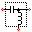
\includegraphics[width=3.5cm]{biast}
\end{center}
\caption{bias t}
\label{fig:biast}
\end{figure}
\FloatBarrier

\subsection{Transformer}
%\addcontentsline{toc}{subsection}{Transformer}

Using the port numbers depicted in fig. \ref{fig:trafo}, the
scattering parameters of an ideal transformer with voltage
transformation ratio $T$ (number of turns) writes as follows.

\begin{equation}
S_{14} = S_{22} = S_{33} = S_{41} = \frac{1}{T^2+1}
\end{equation}
\begin{equation}
S_{12} = -S_{13} = S_{21} = -S_{24} = -S_{31} = S_{34} = -S_{42} = S_{43} = T\cdot S_{22}
\end{equation}
\begin{equation}
S_{11} = S_{23} = S_{32} = S_{44} = T\cdot S_{12}
\end{equation}

\begin{figure}[ht]
\begin{center}
\includegraphics[width=4cm]{trafo}
\end{center}
\caption{transformer}
\label{fig:trafo}
\end{figure}
\FloatBarrier

\subsection{Symmetrical transformer}
%\addcontentsline{toc}{subsection}{Symmetrical transformer}

Using the port numbers depicted in fig. \ref{fig:symtrafo}, the
scattering parameters of an ideal, symmetrical transformer with
voltage transformation ratio (number of turns) $T_1$ and $T_2$,
respectively, writes as follows.

\begin{equation}
denom = T_1^2+T_2^2+T_1^2\cdot T_2^2
\end{equation}
\begin{eqnarray}
S_{11} = S_{66} = \frac{T_2^2}{denom}  &  \qquad S_{16} = S_{61} = 1-S_{11} \\
S_{44} = S_{55} = \frac{T_1^2}{denom}  &  \qquad S_{45} = S_{54} = 1-S_{44} \\
S_{22} = S_{33} = \frac{T_1^2\cdot T_2^2}{denom}  &  \qquad S_{23} = S_{32} = 1-S_{22}
\end{eqnarray}
\begin{equation}
S_{12} = S_{21} = -S_{13} = -S_{31} = -S_{26} = -S_{62} = S_{36} = S_{63}
       = \frac{T_1\cdot T_2^2}{denom}
\end{equation}
\begin{equation}
-S_{24} = -S_{42} = S_{25} = S_{52} = S_{34} = S_{43} = -S_{35} = -S_{53}
       = \frac{T_1^2\cdot T_2}{denom}
\end{equation}
\begin{equation}
-S_{14} = -S_{41} = S_{15} = S_{51} = S_{46} = S_{64} = -S_{56} = -S_{65}
       = \frac{T_1\cdot T_2}{denom}
\end{equation}

\begin{figure}[ht]
\begin{center}
\includegraphics[width=4cm]{symtrafo}
\end{center}
\caption{symmetrical transformer}
\label{fig:symtrafo}
\end{figure}
\FloatBarrier

\subsection{Attenuator}
%\addcontentsline{toc}{subsection}{Attenuator}

The scattering parameters of an ideal attenuator with (power)
attenuation $L$ (loss) (or power gain $G=1/L$) in reference to the
impedance $Z_{ref}$ writes as follows.

\begin{equation}
r = \frac{Z_{ref}-Z_0}{Z_{ref}+Z_0}
\end{equation}
\begin{equation}
S_{11} = S_{22} = \frac{r\cdot(L-1)}{L-r^2} = \frac{r\cdot(1-G)}{1-r^2\cdot G}
\end{equation}
\begin{equation}
S_{12} = S_{21} = \frac{\sqrt{L}\cdot(1-r^2)}{L-r^2} = \frac{\sqrt{G}\cdot(1-r^2)}{1-r^2\cdot G}
\end{equation}

\subsection{Isolator}
%\addcontentsline{toc}{subsection}{Isolator}

An isolator is a one-way two-port, transporting incoming waves
lossless from the input (port 1) to the output (port 2), but consuming
all waves flowing into the output. With the reference impedance of the
input $Z_1$ and the one of the output $Z_2$, the scattering parameters
of an ideal isolator writes as follows.

\begin{equation}
S_{11} = \frac{Z_1-Z_0}{Z_1+Z_0}
\end{equation}
\begin{equation}
S_{12} = 0
\end{equation}
\begin{equation}
S_{22} = \frac{Z_2-Z_0}{Z_2+Z_0}
\end{equation}
\begin{equation}
S_{21} = \sqrt{1-(S_{11})^2}\cdot\sqrt{1-(S_{22})^2}
\end{equation}

\subsection{Circulator}
%\addcontentsline{toc}{subsection}{Circulator}
\label{sec:CirculatorSparameter}

A circulator is a 3-port device, transporting incoming waves lossless
from port 1 to port 2, from port 2 to port 3 and from port 3 to port
1.  In all other directions, there is no energy flow.  With the
reference impedances $Z_1$, $Z_2$ and $Z_3$ for the ports 1, 2 and 3
the scattering matrix of an ideal circulator writes as follows.

\begin{equation}
denom = 1-r_1\cdot r_2\cdot r_3
\end{equation}
\begin{equation}
r_1 = \frac{Z_0-Z_1}{Z_0+Z_1} \qquad,\qquad 
r_2 = \frac{Z_0-Z_2}{Z_0+Z_2} \qquad,\qquad 
r_3 = \frac{Z_0-Z_3}{Z_0+Z_3}
\end{equation}
\begin{equation}
S_{11} = \frac{r_2\cdot r_3 - r_1}{denom} \qquad,\qquad 
S_{22} = \frac{r_1\cdot r_3 - r_2}{denom} \qquad,\qquad 
S_{33} = \frac{r_1\cdot r_2 - r_3}{denom}
\end{equation}
\begin{equation}
S_{12} = \sqrt{\frac{Z_2}{Z_1}}\cdot\frac{Z_1+Z_0}{Z_2+Z_0}\cdot\frac{r_3\cdot(1-r_1^2)}{denom}
\qquad,\qquad 
S_{13} = \sqrt{\frac{Z_3}{Z_1}}\cdot\frac{Z_1+Z_0}{Z_3+Z_0}\cdot\frac{1-r_1^2}{denom}
\end{equation}
\begin{equation}
S_{21} = \sqrt{\frac{Z_1}{Z_2}}\cdot\frac{Z_2+Z_0}{Z_1+Z_0}\cdot\frac{1-r_2^2}{denom}
\qquad,\qquad 
S_{23} = \sqrt{\frac{Z_3}{Z_2}}\cdot\frac{Z_2+Z_0}{Z_3+Z_0}\cdot\frac{r_1\cdot(1-r_2^2)}{denom}
\end{equation}
\begin{equation}
S_{31} = \sqrt{\frac{Z_1}{Z_3}}\cdot\frac{Z_3+Z_0}{Z_1+Z_0}\cdot\frac{r_2\cdot(1-r_3^2)}{denom}
\qquad,\qquad 
S_{32} = \sqrt{\frac{Z_2}{Z_3}}\cdot\frac{Z_3+Z_0}{Z_2+Z_0}\cdot\frac{1-r_3^2}{denom}
\end{equation}

\subsection{Phase shifter}
%\addcontentsline{toc}{subsection}{Phase shifter}

The scattering parameters of an ideal phase shifter with phase shift
$\phi$ and reference impedance $Z_{ref}$ writes as follows.

\begin{equation}
r = \frac{Z_{ref}-Z_0}{Z_{ref}+Z_0}
\end{equation}
\begin{equation}
S_{11} = S_{22} = \frac{r\cdot\left(1-\exp\left(j\cdot 2\phi\right)\right)}{1-r^2\cdot\exp\left(j\cdot 2\phi\right)}
\end{equation}
\begin{equation}
S_{12} = S_{21} = \frac{(1-r^2)\cdot\exp\left(j\cdot\phi\right)}{1-r^2\cdot\exp\left(j\cdot 2\phi\right)}
\end{equation}


\subsection{Gyrator}
%\addcontentsline{toc}{subsection}{Gyrator}

A gyrator is an impedance inverter.  Thus, for example, it converts a
capacitance into an inductance and vice versa.  The scattering matrix
of an ideal gyrator with the ratio $R$ writes as follows.

\begin{equation}
r = \frac{R}{Z_{ref}} = \frac{1}{G\cdot Z_{ref}}
\end{equation}
\begin{equation}
S_{11} = S_{22} = S_{33} = S_{44} = \frac{R^2}{4\cdot Z_{ref}^2 + R^2} = \frac{r^2}{r^2+4}
\end{equation}
\begin{equation}
S_{14} = S_{23} = S_{32} = S_{41} = 1-S_{11}
\end{equation}
\begin{equation}
S_{12} = -S_{13} = -S_{21} = S_{24} = S_{31} = -S_{34} = -S_{42} = S_{43} = \frac{2\cdot r}{r^2+4}
\end{equation}

\subsection{Voltage and current sources}
%\addcontentsline{toc}{subsection}{Voltage and current sources}

All voltage sources (AC and DC) are short circuits and therefore their
S-parameter matrix equals the one of the DC block.  All current
sources are open circuits and therefore their S-parameter matrix
equals the one of the DC feed.

\subsection{Controlled voltage and current sources}
%\addcontentsline{toc}{subsection}{Controlled voltage and current sources}

The scattering matrix of the voltage controlled current source
depicted in fig. \ref{fig:xCCS} (left) writes as follows ($\tau$ is
time delay).

\begin{equation}
S_{11} = S_{22} = S_{33} = S_{44} = 1
\end{equation}
\begin{equation}
S_{12} = S_{13} = S_{14} = S_{23} = S_{32} = S_{41} = S_{42} = S_{43} = 0
\end{equation}
\begin{equation}
S_{21} = S_{34} = 2\cdot G\cdot \exp\left(j\pi-j\omega\tau\right)
\end{equation}
\begin{equation}
S_{24} = S_{31} = 2\cdot G\cdot \exp\left(-j\omega\tau\right)
\end{equation}

\begin{figure}[ht]
\begin{center}
\includegraphics[width=8cm]{xCCS}
\end{center}
\caption{voltage controlled current source (left) and current controlled current source (right)}
\label{fig:xCCS}
\end{figure}
\FloatBarrier

The scattering matrix of the current controlled current source
depicted in fig. \ref{fig:xCCS} (right) writes as follows ($\tau$ is
time delay).

\begin{equation}
S_{14} = S_{22} = S_{33} = S_{41} = 1
\end{equation}
\begin{equation}
S_{11} = S_{12} = S_{13} = S_{23} = S_{32} = S_{42} = S_{43} = S_{44} = 0
\end{equation}
\begin{equation}
S_{21} = S_{34} = G\cdot \exp\left(j\pi-j\omega\tau\right)
\end{equation}
\begin{equation}
S_{24} = S_{31} = G\cdot \exp\left(-j\omega\tau\right)
\end{equation}

The scattering matrix of the voltage controlled voltage source
depicted in fig. \ref{fig:xCVS} (left) writes as follows ($\tau$ is
time delay).

\begin{equation}
S_{11} = S_{23} = S_{32} = S_{44} = 1
\end{equation}
\begin{equation}
S_{12} = S_{13} = S_{14} = S_{22} = S_{33} = S_{41} = S_{42} = S_{43} = 0
\end{equation}
\begin{equation}
S_{21} = S_{34} = G\cdot \exp\left(-j\omega\tau\right)
\end{equation}
\begin{equation}
S_{24} = S_{31} = G\cdot \exp\left(j\pi-j\omega\tau\right)
\end{equation}

\begin{figure}[ht]
\begin{center}
\includegraphics[width=8cm]{xCVS}
\end{center}
\caption{voltage controlled voltage source (left) and current controlled voltage source (right)}
\label{fig:xCVS}
\end{figure}
\FloatBarrier

The scattering matrix of the current controlled voltage source
depicted in fig. \ref{fig:xCVS} (right) writes as follows ($\tau$ is
time delay).

\begin{equation}
S_{14} = S_{23} = S_{32} = S_{41} = 1
\end{equation}
\begin{equation}
S_{11} = S_{12} = S_{13} = S_{22} = S_{33} = S_{42} = S_{43} = S_{44} = 0
\end{equation}
\begin{equation}
S_{21} = S_{34} = \frac{G}{2}\cdot \exp\left(-j\omega\tau\right)
\end{equation}
\begin{equation}
S_{24} = S_{31} = \frac{G}{2}\cdot \exp\left(j\pi-j\omega\tau\right)
\end{equation}

\subsection{Transmission Line}
%\addcontentsline{toc}{subsection}{Transmission Line}

The scattering matrix of an ideal, lossless transmission line with
impedance $Z$ and electrical length $l$ writes as follows.

\begin{equation}
r = \frac{Z-Z_0}{Z+Z_0}
\end{equation}
\begin{equation}
p = \exp\left(-j\omega\frac{l}{c_0}\right)
\end{equation}
\begin{equation}
S_{11} = S_{22} = \frac{r\cdot(1-p^2)}{1-r^2\cdot p^2} \qquad,\qquad
S_{12} = S_{21} = \frac{p\cdot(1-r^2)}{1-r^2\cdot p^2}
\end{equation}

With $c_0$ = 299 792 458 m/s being the vacuum light velocity.

\subsection{S-parameter container with additional reference port}
%\addcontentsline{toc}{subsection}{S-parameter container with additional reference port}
\label{sec:spfile}

\begin{figure}[ht]
\begin{center}
\includegraphics[width=0.6\linewidth]{spfile}
\end{center}
\caption{S-parameter container}
\label{fig:spfile}
\end{figure}
\FloatBarrier

In order to extend a $m - 1$-port to have a S-parameter device with
$m$ ports assuming that the original reference port had a reflection
coefficient $\Gamma_m$ the new S-parameters are according to
T. O. Grosch and L. A. Carpenter \cite{Grosch}:
\begin{align}
S_{mm} &= \dfrac{2 - \Gamma_m - m + {\displaystyle\sum_{i=1}^{m-1}}\, {\displaystyle\sum_{j=1}^{m-1}} S'_{ij}}{1 - m\cdot \Gamma_m - {\displaystyle\sum_{i=1}^{m-1}}\, {\displaystyle\sum_{j=1}^{m-1}} S'_{ij}}\\
S_{im} &= \left(\dfrac{1 - \Gamma_m\cdot S_{mm}}{1 - \Gamma_m}\right)\cdot \left(1 - \sum_{j=1}^{m-1} S'_{ij}\right) &
\textrm{ for } i = 1,2 \ldots m - 1\\
S_{mj} &= \left(\dfrac{1 - \Gamma_m\cdot S_{mm}}{1 - \Gamma_m}\right)\cdot \left(1 - \sum_{i=1}^{m-1} S'_{ij}\right) &
\textrm{ for } j = 1,2 \ldots m - 1\\
S_{ij} &= S'_{ij} - \left(\dfrac{\Gamma_m\cdot S_{im}\cdot S_{mj}}{1 - \Gamma_m\cdot S_{mm}}\right) &
\textrm{ for } i,j = 1,2 \ldots m - 1
\end{align}

If the reference port has been ground potential, then $\Gamma_m$
simply folds to -1.  The reverse transformation by connecting a
termination with a reflection coefficient of $\Gamma_m$ to the $m$th
port writes as follows.
\begin{equation}
S'_{ij} = S_{ij} + \left(\dfrac{\Gamma_m\cdot S_{im}\cdot S_{mj}}{1 - \Gamma_m\cdot S_{mm}}\right)
\;\;\;\; \textrm{ for } i,j = 1,2 \ldots m - 1
\end{equation}
